\definecolor{opt}{HTML}{51B824}
\definecolor{amm}{HTML}{CC0000}

\section{Cruscotto di valutazione della qualità}
\subsection{Qualità del processo di Analisi dei requisiti}
\subsubsection{1M-CRO - Copertura dei requisiti obbligatori}
%--------- GRAFICO -----------%
\begin{figure*}[!h]
    \centering
    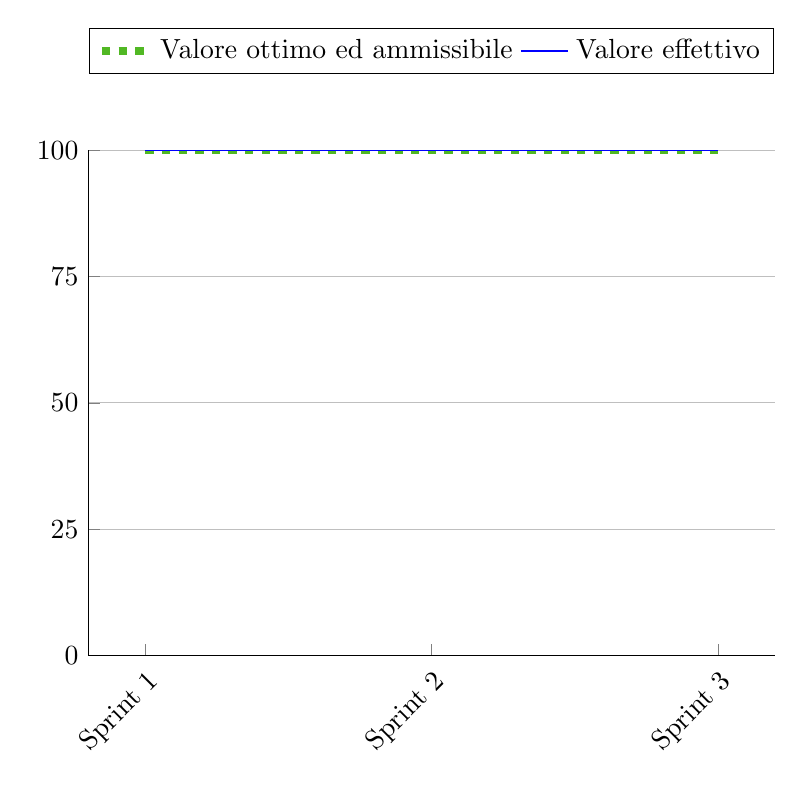
\begin{tikzpicture}
        \begin{axis}[
            width  = 0.85*\textwidth,
            height = 8cm,
            ymajorgrids = true,
            symbolic x coords={Sprint 1, Sprint 2, Sprint 3},
            xtick = data,
            ytick = {0, 25, 50, 75, 100},
            ymin=0, ymax=100,
            axis lines*=left,
            legend cell align=left,
            legend style={
                at={(0.5,1.15)},
                anchor=south,
                column sep=0.1ex,
                legend columns=3
            },      
            xticklabel style={rotate=45, anchor=north east, yshift=0ex, xshift=0ex}
            ]
            \addplot[color=opt, style={dashed, line width=3pt}, mark=none] coordinates {(Sprint 1, 100) (Sprint 2, 100) (Sprint 3, 100)};
            \addplot[color=blue, style={line width=1pt}, mark=none] coordinates {(Sprint 1, 100) (Sprint 2, 100) (Sprint 3, 100)};
            \legend{Valore ottimo ed ammissibile, Valore effettivo}
        \end{axis}
    \end{tikzpicture}
    \caption{Percentuale di copertura dei requisiti obbligatori}
    \label{fig:1}
\end{figure*}
%--------- FINE GRAFICO -----------%
%\textbf{RTB} \\
% TODO considerazioni finali per RTB \\
%\textbf{PB} \\
% TODO considerazioni finali per PB

\newpage
\subsubsection{2M-CRD - Copertura dei requisiti desiderabili}
%--------- GRAFICO -----------%
\begin{figure*}[!h]
    \centering
    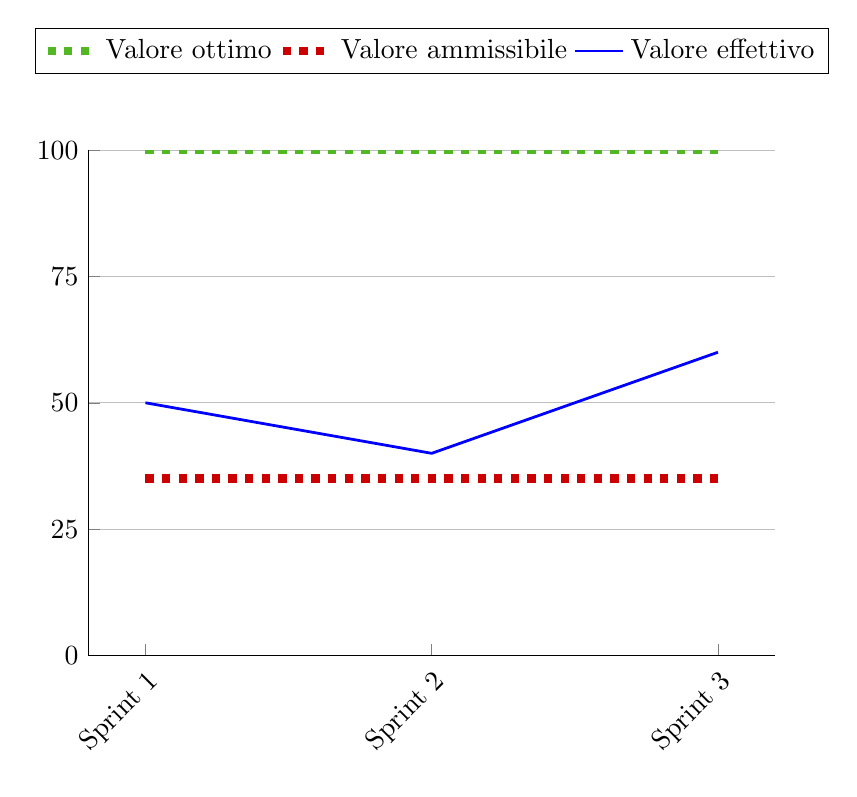
\begin{tikzpicture}
        \begin{axis}[
            width  = 0.85*\textwidth,
            height = 8cm,
            ymajorgrids = true,
            symbolic x coords={Sprint 1, Sprint 2, Sprint 3},
            xtick = data,
            ytick = {0, 25, 50, 75, 100},
            ymin=0, ymax=100,
            axis lines*=left,
            legend cell align=left,
            legend style={
                at={(0.5,1.15)},
                anchor=south,
                column sep=0.1ex,
                legend columns=3
            },      
            xticklabel style={rotate=45, anchor=north east, yshift=0ex, xshift=0ex}
            ]
            \addplot[color=opt, style={dashed, line width=3pt}, mark=none] coordinates {(Sprint 1, 100) (Sprint 2, 100) (Sprint 3, 100)};
            \addplot[color=amm, style={dashed, line width=3pt}, mark=none] coordinates {(Sprint 1, 35) (Sprint 2, 35) (Sprint 3, 35)};
            \addplot[color=blue, style={line width=1pt}, mark=none] coordinates {(Sprint 1, 50) (Sprint 2, 40) (Sprint 3, 60)};
            \legend{Valore ottimo, Valore ammissibile, Valore effettivo}
        \end{axis}
    \end{tikzpicture}
    \caption{Percentuale di copertura dei requisiti desiderabili}
    \label{fig:2}
\end{figure*}
%--------- FINE GRAFICO -----------%
%\textbf{RTB} \\
% TODO considerazioni finali per RTB \\
%\textbf{PB} \\
% TODO considerazioni finali per PB

\newpage
\subsubsection{3M-CROP - Copertura dei requisiti opzionali}
%--------- GRAFICO -----------%
\begin{figure*}[!h]
    \centering
    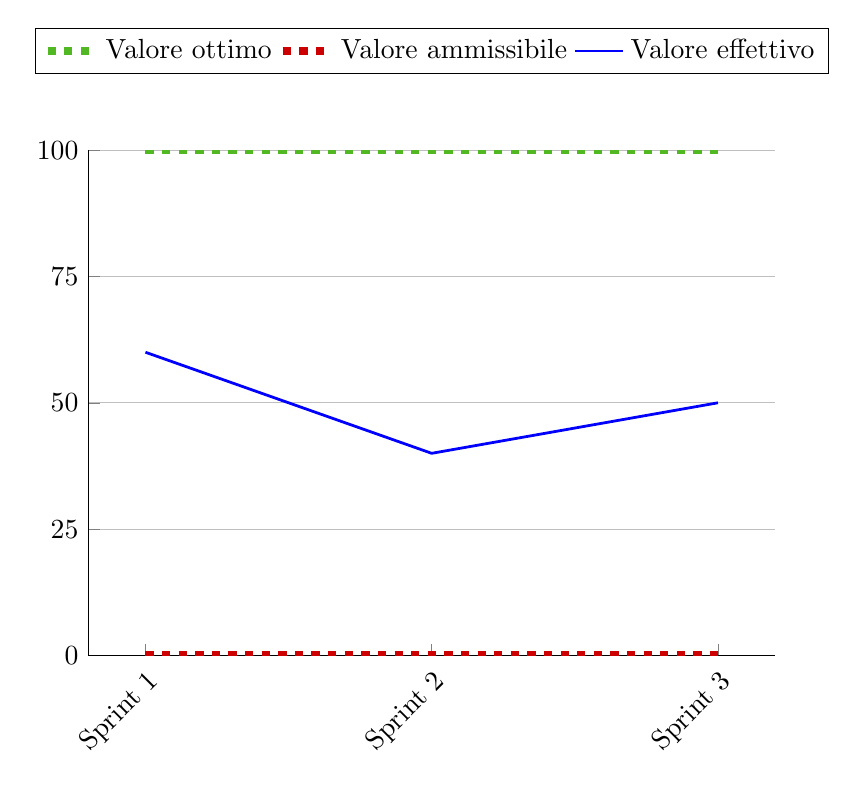
\begin{tikzpicture}
        \begin{axis}[
            width  = 0.85*\textwidth,
            height = 8cm,
            ymajorgrids = true,
            symbolic x coords={Sprint 1, Sprint 2, Sprint 3},
            xtick = data,
            ytick = {0, 25, 50, 75, 100},
            ymin=0, ymax=100,
            axis lines*=left,
            legend cell align=left,
            legend style={
                at={(0.5,1.15)},
                anchor=south,
                column sep=0.1ex,
                legend columns=3
            },      
            xticklabel style={rotate=45, anchor=north east, yshift=0ex, xshift=0ex}
            ]
            \addplot[color=opt, style={dashed, line width=3pt}, mark=none] coordinates {(Sprint 1, 100) (Sprint 2, 100) (Sprint 3, 100)};
            \addplot[color=amm, style={dashed, line width=3pt}, mark=none] coordinates {(Sprint 1, 0) (Sprint 2, 0) (Sprint 3, 0)};
            \addplot[color=blue, style={line width=1pt}, mark=none] coordinates {(Sprint 1, 60) (Sprint 2, 40) (Sprint 3, 50)};
            \legend{Valore ottimo, Valore ammissibile, Valore effettivo}
        \end{axis}
    \end{tikzpicture}
    \caption{Percentuale di copertura dei requisiti opzionali}
    \label{fig:3}
\end{figure*}
%--------- FINE GRAFICO -----------%
%\textbf{RTB} \\
% TODO considerazioni finali per RTB \\
%\textbf{PB} \\
% TODO considerazioni finali per PB

\newpage
\subsection{Qualità del processo di Fornitura}
\subsubsection{9M-EV - Earned Value (EV) e 10M-PV - Planned Value (PV)}
%--------- GRAFICO -----------%
\begin{figure*}[!h]
    \centering
    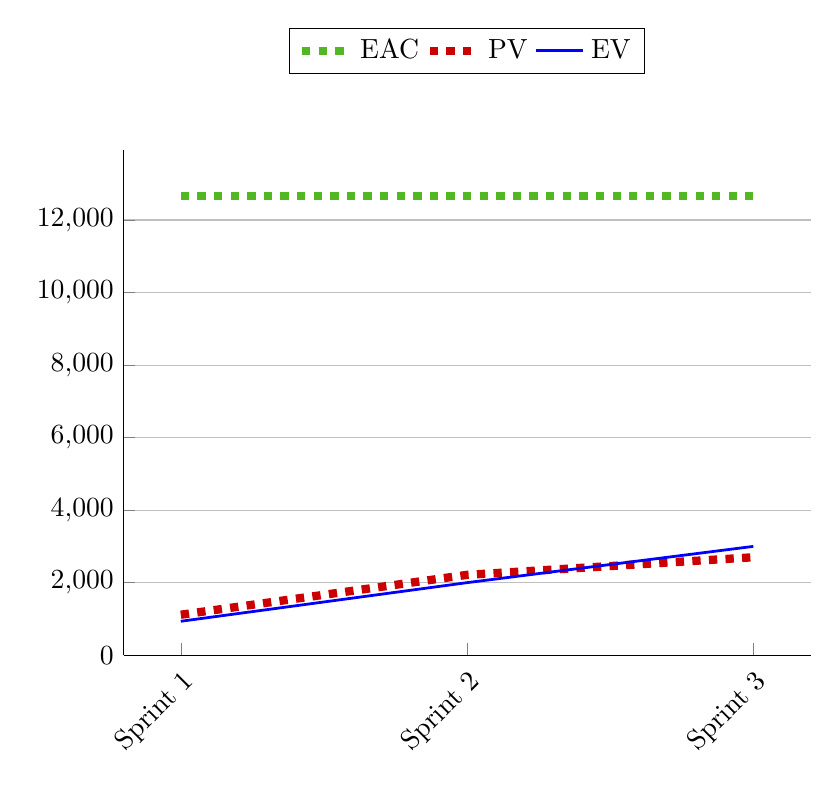
\begin{tikzpicture}
        %da chiedere se è giusta questa interpretazione
        \begin{axis}[
            width  = 0.85*\textwidth,
            height = 8cm,
            ymajorgrids = true,
            symbolic x coords={Sprint 1, Sprint 2, Sprint 3},
            xtick = data,
            ymin=0,
            axis lines*=left,
            legend cell align=left,
            legend style={
                at={(0.5,1.15)},
                anchor=south,
                column sep=0.1ex,
                legend columns=3
            },      
            xticklabel style={rotate=45, anchor=north east, yshift=0ex, xshift=0ex},
            scaled y ticks = false,
            yticklabel style={/pgf/number format/fixed}
            ]
            \addplot[color=opt, style={dashed, line width=3pt}, mark=none] coordinates {(Sprint 1, 12670) (Sprint 2, 12670) (Sprint 3, 12670)}; % TODO mettere valori corretti EAC
            \addplot[color=amm, style={dashed, line width=3pt}, mark=none] coordinates {(Sprint 1, 1115) (Sprint 2, 2215) (Sprint 3, 2700)}; % TODO mettere valori corretti PV
            \addplot[color=blue, style={line width=1pt}, mark=none] coordinates {(Sprint 1, 935) (Sprint 2, 2000) (Sprint 3, 3000)}; % TODO mettere valori corretti EV
            \legend{EAC, PV, EV}
        \end{axis}
    \end{tikzpicture}
    \caption{Proiezione del PV e dell'EV}
    \label{fig:4}
\end{figure*}
%--------- FINE GRAFICO -----------%
%\textbf{RTB} \\
% TODO considerazioni finali per RTB \\
%\textbf{PB} \\
% TODO considerazioni finali per PB

\newpage
\subsubsection{11M-AC - Actual Cost (AC) e 14M-ETC - Estimate to Complete (ETC)}
% da controllare
%--------- GRAFICO -----------%
\begin{figure*}[!h]
    \centering
    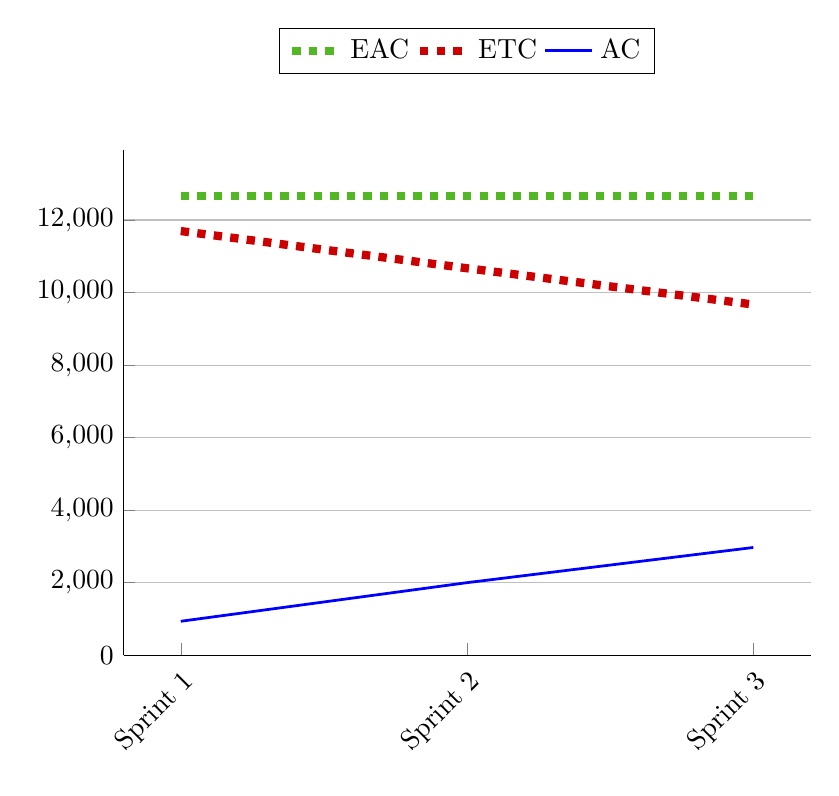
\begin{tikzpicture}
        \begin{axis}[
            width  = 0.85*\textwidth,
            height = 8cm,
            ymajorgrids = true,
            symbolic x coords={Sprint 1, Sprint 2, Sprint 3},
            xtick = data,
            ymin=0,
            axis lines*=left,
            legend cell align=left,
            legend style={
                at={(0.5,1.15)},
                anchor=south,
                column sep=0.1ex,
                legend columns=3
            },      
            xticklabel style={rotate=45, anchor=north east, yshift=0ex, xshift=0ex},
            scaled y ticks = false,
            yticklabel style={/pgf/number format/fixed}
            ]
            \addplot[color=opt, style={dashed, line width=3pt}, mark=none] coordinates {(Sprint 1, 12670) (Sprint 2, 12670) (Sprint 3, 12670)}; 
            \addplot[color=amm, style={dashed, line width=3pt}, mark=none] coordinates {(Sprint 1, 11695) (Sprint 2, 10670) (Sprint 3, 9670)};
            \addplot[color=blue, style={line width=1pt}, mark=none] coordinates {(Sprint 1, 935) (Sprint 2, 2000) (Sprint 3, 2970)};
            \legend{EAC, ETC, AC}
        \end{axis}
    \end{tikzpicture}
    \caption{Percentuale di copertura dei requisiti obbligatori per ogni sprint}
    \label{fig:5}
\end{figure*}
%--------- FINE GRAFICO -----------%
%\textbf{RTB} \\
% TODO considerazioni finali per RTB \\
%\textbf{PB} \\
% TODO considerazioni finali per PB

\newpage
\subsubsection{12M-CV - Cost Variance (CV) e 33M-SV - Schedule Variance (SV)}
%--------- GRAFICO -----------%
\begin{figure*}[!h]
    \centering
    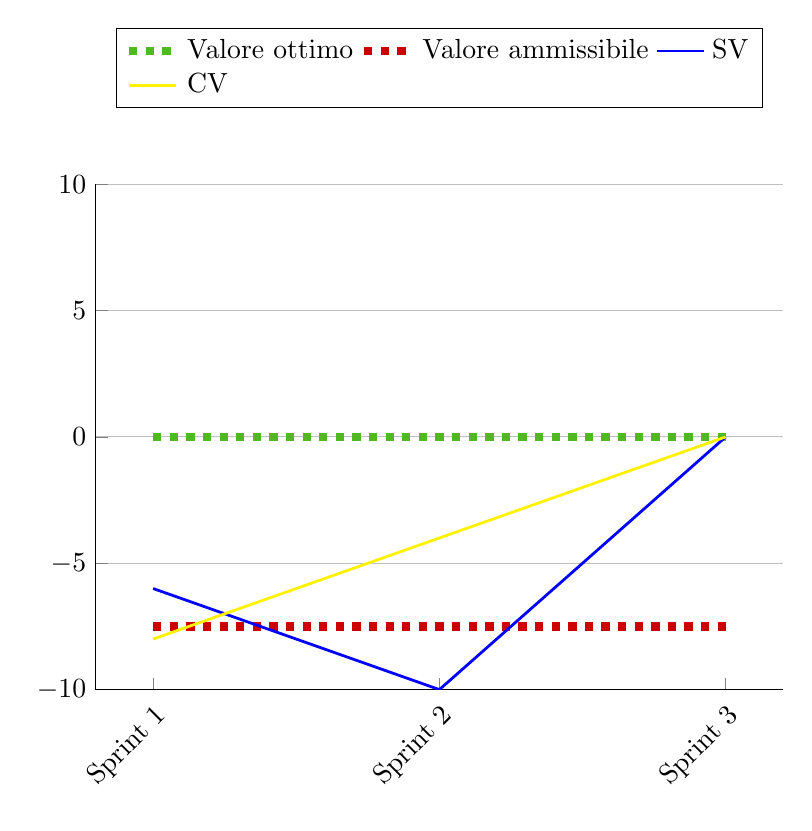
\begin{tikzpicture}
        \begin{axis}[
            width  = 0.85*\textwidth,
            height = 8cm,
            ymajorgrids = true,
            symbolic x coords={Sprint 1, Sprint 2, Sprint 3},
            xtick = data,
            ymin=-10, ymax=10,
            axis lines*=left,
            legend cell align=left,
            legend style={
                at={(0.5,1.15)},
                anchor=south,
                column sep=0.1ex,
                legend columns=3
            },      
            xticklabel style={rotate=45, anchor=north east, yshift=0ex, xshift=0ex}
            ]
            \addplot[color=opt, style={dashed, line width=3pt}, mark=none] coordinates {(Sprint 1, 0) (Sprint 2, 0) (Sprint 3, 0)};
            \addplot[color=amm, style={dashed, line width=3pt}, mark=none] coordinates {(Sprint 1, -7.5) (Sprint 2, -7.5) (Sprint 3, -7.5)};
            \addplot[color=blue, style={line width=1pt}, mark=none] coordinates {(Sprint 1, -6) (Sprint 2, -10) (Sprint 3, 0)}; % TODO mettere valori corretti SV terzo periodo
            \addplot[color=yellow, style={line width=1pt}, mark=none] coordinates {(Sprint 1, -8) (Sprint 2, -4) (Sprint 3, 0)}; % TODO mettere valori corretti CV terzo periodo
            \legend{Valore ottimo, Valore ammissibile, SV, CV}
        \end{axis}
    \end{tikzpicture}
    \caption{Andamento percentuale di SV e CV}
    \label{fig:6}
\end{figure*}
%--------- FINE GRAFICO -----------%
%\textbf{RTB} \\
% TODO considerazioni finali per RTB \\
%\textbf{PB} \\
% TODO considerazioni finali per PB

\newpage
\subsubsection{13M-EAC - Estimated at Completion (EAC)}
Quanti soldi prevediamo di spendere per la fine del progetto
%--------- GRAFICO -----------%
\begin{figure*}[!h]
    \centering
    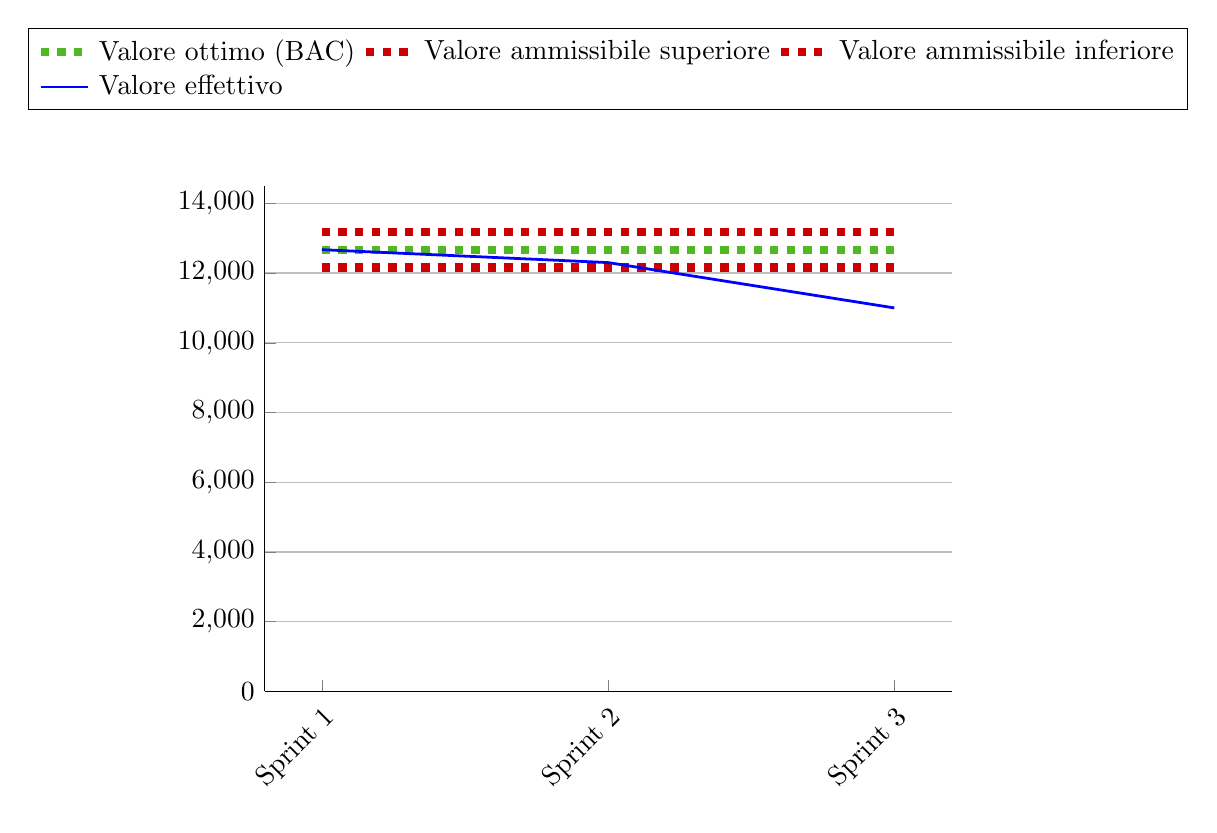
\begin{tikzpicture}
        \begin{axis}[
            width  = 0.85*\textwidth,
            height = 8cm,
            ymajorgrids = true,
            symbolic x coords={Sprint 1, Sprint 2, Sprint 3},
            xtick = data,
            ymin=0,
            axis lines*=left,
            legend cell align=left,
            legend style={
                at={(0.5,1.15)},
                anchor=south,
                column sep=0.1ex,
                legend columns=3
            },      
            xticklabel style={rotate=45, anchor=north east, yshift=0ex, xshift=0ex},
            scaled y ticks = false,
            yticklabel style={/pgf/number format/fixed}
            ]
            \addplot[color=opt, style={dashed, line width=3pt}, mark=none] coordinates {(Sprint 1, 12670) (Sprint 2, 12670) (Sprint 3, 12670)}; % TODO mettere valori corretti BAC
            \addplot[color=amm, style={dashed, line width=3pt}, mark=none] coordinates {(Sprint 1, 13177) (Sprint 2, 13177) (Sprint 3, 13177)}; % TODO mettere valori corretti BAC + 4%
            \addplot[color=amm, style={dashed, line width=3pt}, mark=none] coordinates {(Sprint 1, 12162) (Sprint 2, 12162) (Sprint 3, 12162)}; % TODO mettere valori corretti BAC - 4%
            \addplot[color=blue, style={line width=1pt}, mark=none] coordinates {(Sprint 1, 12670) (Sprint 2, 12300) (Sprint 3, 11000)}; % TODO mettere valori corretti EAC
            \legend{Valore ottimo (BAC), Valore ammissibile superiore, Valore ammissibile inferiore, Valore effettivo}
        \end{axis}
    \end{tikzpicture}
    \caption{Percentuale di copertura dei requisiti obbligatori per ogni sprint}
    \label{fig:7}
\end{figure*}
%--------- FINE GRAFICO -----------%
%\textbf{RTB} \\
% TODO considerazioni finali per RTB \\
%\textbf{PB} \\
% TODO considerazioni finali per PB

\newpage
\subsection{Qualità del processo di Documentazione}
\subsubsection{22M-IG - Indice Gulpease}
%--------- GRAFICO -----------%
\begin{figure*}[!h]
    \centering
    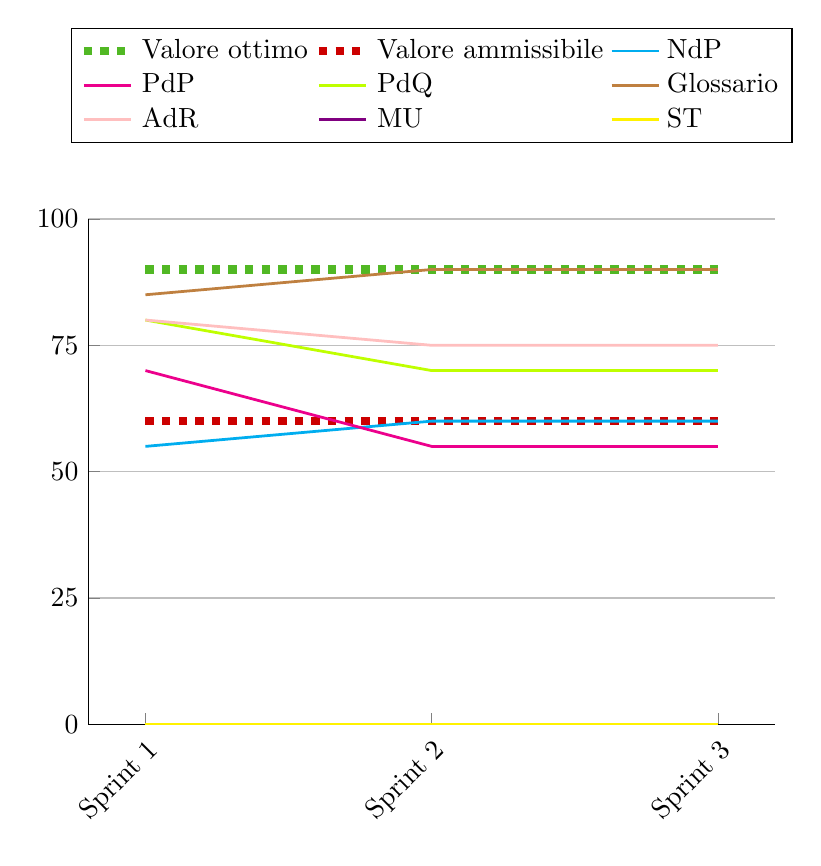
\begin{tikzpicture}
        \begin{axis}[
            width  = 0.85*\textwidth,
            height = 8cm,
            ymajorgrids = true,
            symbolic x coords={Sprint 1, Sprint 2, Sprint 3},
            xtick = data,
            ytick = {0, 25, 50, 75, 100},
            ymin=0, ymax=100,
            axis lines*=left,
            legend cell align=left,
            legend style={
                at={(0.5,1.15)},
                anchor=south,
                column sep=0.1ex,
                legend columns=3
            },           
            xticklabel style={rotate=45, anchor=north east, yshift=0ex, xshift=0ex}
            ]
            \addplot[color=opt, style={dashed, line width=3pt}, mark=none] coordinates {(Sprint 1, 90) (Sprint 2, 90) (Sprint 3, 90)};
            \addplot[color=amm, style={dashed, line width=3pt}, mark=none] coordinates {(Sprint 1, 60) (Sprint 2, 60) (Sprint 3, 60)};
            \addplot[color=cyan, style={line width=1pt}, mark=none] coordinates {(Sprint 1, 55) (Sprint 2, 60) (Sprint 3, 60)}; % TODO mettere valori corretti NdP
            \addplot[color=magenta, style={line width=1pt}, mark=none] coordinates {(Sprint 1, 70) (Sprint 2, 55) (Sprint 3, 55)}; % TODO mettere valori corretti PdP
            \addplot[color=lime, style={line width=1pt}, mark=none] coordinates {(Sprint 1, 80) (Sprint 2, 70) (Sprint 3, 70)}; % TODO mettere valori corretti PdQ
            \addplot[color=brown, style={line width=1pt}, mark=none] coordinates {(Sprint 1, 85) (Sprint 2, 90) (Sprint 3, 90)}; % TODO mettere valori corretti Glossario
            \addplot[color=pink, style={line width=1pt}, mark=none] coordinates {(Sprint 1, 80) (Sprint 2, 75) (Sprint 3, 75)}; % TODO mettere valori corretti AdR
            \addplot[color=violet, style={line width=1pt}, mark=none] coordinates {(Sprint 1, 0) (Sprint 2, 0) (Sprint 3, 0)}; % TODO mettere valori corretti MU
            \addplot[color=yellow, style={line width=1pt}, mark=none] coordinates {(Sprint 1, 0) (Sprint 2, 0) (Sprint 3, 0)}; % TODO mettere valori corretti ST
            \legend{Valore ottimo, Valore ammissibile, NdP, PdP, PdQ, Glossario, AdR, MU, ST}
        \end{axis}
    \end{tikzpicture}
    \caption{Andamento indice di Gulpease per ciascun documento}
    \label{fig:8}
\end{figure*}
%--------- FINE GRAFICO -----------%
%\textbf{RTB} \\
% TODO considerazioni finali per RTB \\
%\textbf{PB} \\
% TODO considerazioni finali per PB

\newpage
\subsubsection{23M-CO - Correttezza Ortografica}
%--------- GRAFICO -----------%
\begin{figure*}[!h]
    \centering
    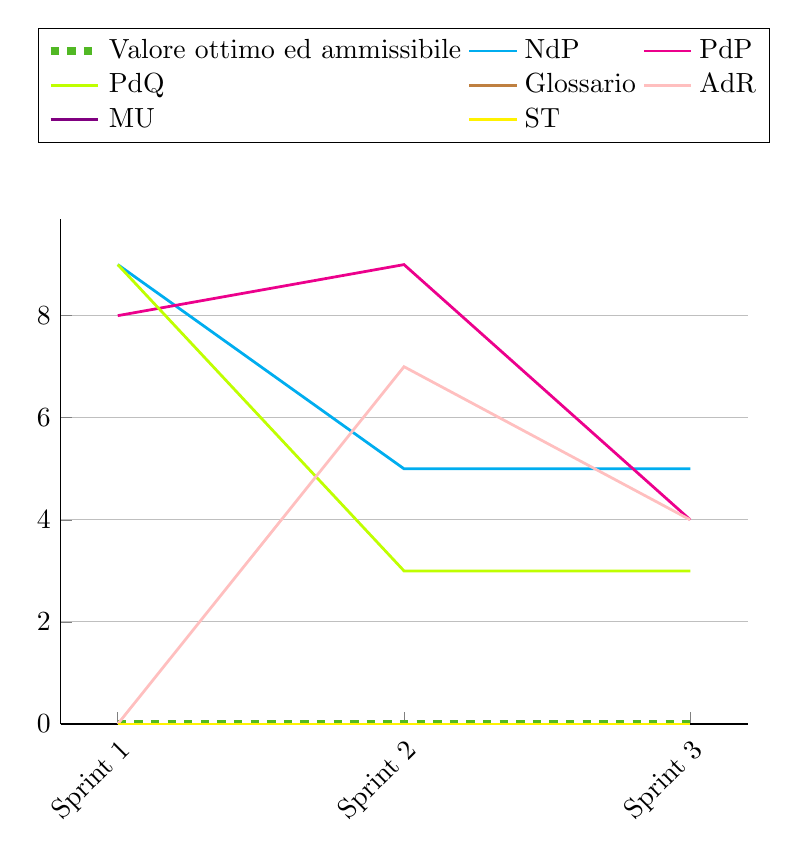
\begin{tikzpicture}
        \begin{axis}[
            width  = 0.85*\textwidth,
            height = 8cm,
            ymajorgrids = true,
            symbolic x coords={Sprint 1, Sprint 2, Sprint 3},
            xtick = data,
            ymin=0,
            axis lines*=left,
            legend cell align=left,
            legend style={
                at={(0.5,1.15)},
                anchor=south,
                column sep=0.1ex,
                legend columns=3
            },           
            xticklabel style={rotate=45, anchor=north east, yshift=0ex, xshift=0ex}
            ]
            \addplot[color=opt, style={dashed, line width=3pt}, mark=none] coordinates {(Sprint 1, 0) (Sprint 2, 0) (Sprint 3, 0)};
            \addplot[color=cyan, style={line width=1pt}, mark=none] coordinates {(Sprint 1, 9) (Sprint 2, 5) (Sprint 3, 5)}; % TODO mettere valori corretti NdP
            \addplot[color=magenta, style={line width=1pt}, mark=none] coordinates {(Sprint 1, 8) (Sprint 2, 9) (Sprint 3, 4)}; % TODO mettere valori corretti PdP
            \addplot[color=lime, style={line width=1pt}, mark=none] coordinates {(Sprint 1, 9) (Sprint 2, 3) (Sprint 3, 3)}; % TODO mettere valori corretti PdQ
            \addplot[color=brown, style={line width=1pt}, mark=none] coordinates {(Sprint 1, 0) (Sprint 2, 0) (Sprint 3, 0)}; % TODO mettere valori corretti Glossario
            \addplot[color=pink, style={line width=1pt}, mark=none] coordinates {(Sprint 1, 0) (Sprint 2, 7) (Sprint 3, 4)}; % TODO mettere valori corretti AdR
            \addplot[color=violet, style={line width=1pt}, mark=none] coordinates {(Sprint 1, 0) (Sprint 2, 0) (Sprint 3, 0)}; % TODO mettere valori corretti MU
            \addplot[color=yellow, style={line width=1pt}, mark=none] coordinates {(Sprint 1, 0) (Sprint 2, 0) (Sprint 3, 0)}; % TODO mettere valori corretti ST
            \legend{Valore ottimo ed ammissibile, NdP, PdP, PdQ, Glossario, AdR, MU, ST}
        \end{axis}
    \end{tikzpicture}
    \caption{Errori ortografici per ciascun documento}
    \label{fig:9}
\end{figure*}
%--------- FINE GRAFICO -----------%
%\textbf{RTB} \\
% TODO considerazioni finali per RTB \\
%\textbf{PB} \\
% TODO considerazioni finali per PB

\newpage
\subsection{Qualità del processo di Verifica}
\subsubsection{24M-CC - Code coverage}
%Da qui in poi byteops fanno da "periodo 6"
%--------- GRAFICO -----------%
\begin{figure*}[!h]
    \centering
    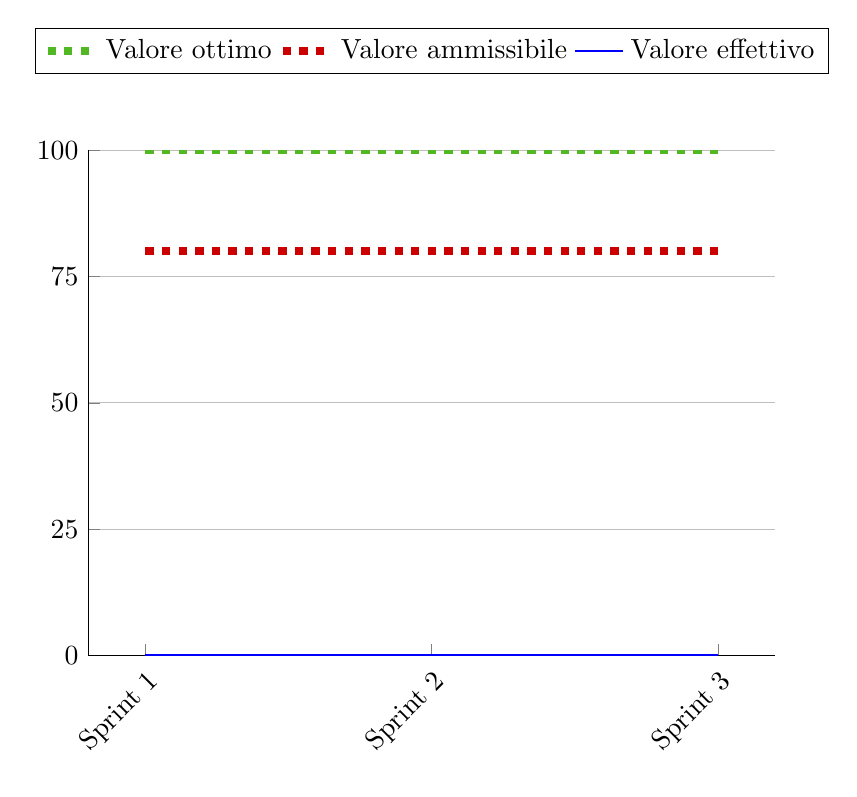
\begin{tikzpicture}
        \begin{axis}[
            width  = 0.85*\textwidth,
            height = 8cm,
            ymajorgrids = true,
            symbolic x coords={Sprint 1, Sprint 2, Sprint 3},
            xtick = data,
            ytick = {0, 25, 50, 75, 100},
            ymin=0, ymax=100,
            axis lines*=left,
            legend cell align=left,
            legend style={
                at={(0.5,1.15)},
                anchor=south,
                column sep=0.1ex,
                legend columns=-1
            },           
            xticklabel style={rotate=45, anchor=north east, yshift=0ex, xshift=0ex}
            ]
            \addplot[color=opt, style={dashed, line width=3pt}, mark=none] coordinates {(Sprint 1, 100) (Sprint 2, 100) (Sprint 3, 100)};
            \addplot[color=amm, style={dashed, line width=3pt}, mark=none] coordinates {(Sprint 1, 80) (Sprint 2, 80) (Sprint 3, 80)};
            \addplot[color=blue, style={line width=1pt}, mark=none] coordinates {(Sprint 1, 0) (Sprint 2, 0) (Sprint 3, 0)};
            \legend{Valore ottimo, Valore ammissibile, Valore effettivo}
        \end{axis}
    \end{tikzpicture}
    \caption{Percentuale di code coverage dei test implementati}
    \label{fig:10}
\end{figure*}
%--------- FINE GRAFICO -----------%
%\textbf{RTB} \\
% TODO considerazioni finali per RTB \\
%\textbf{PB} \\
% TODO considerazioni finali per PB

\newpage
\subsubsection{25M-BC - Branch coverage}
%--------- GRAFICO -----------%
\begin{figure*}[!h]
    \centering
    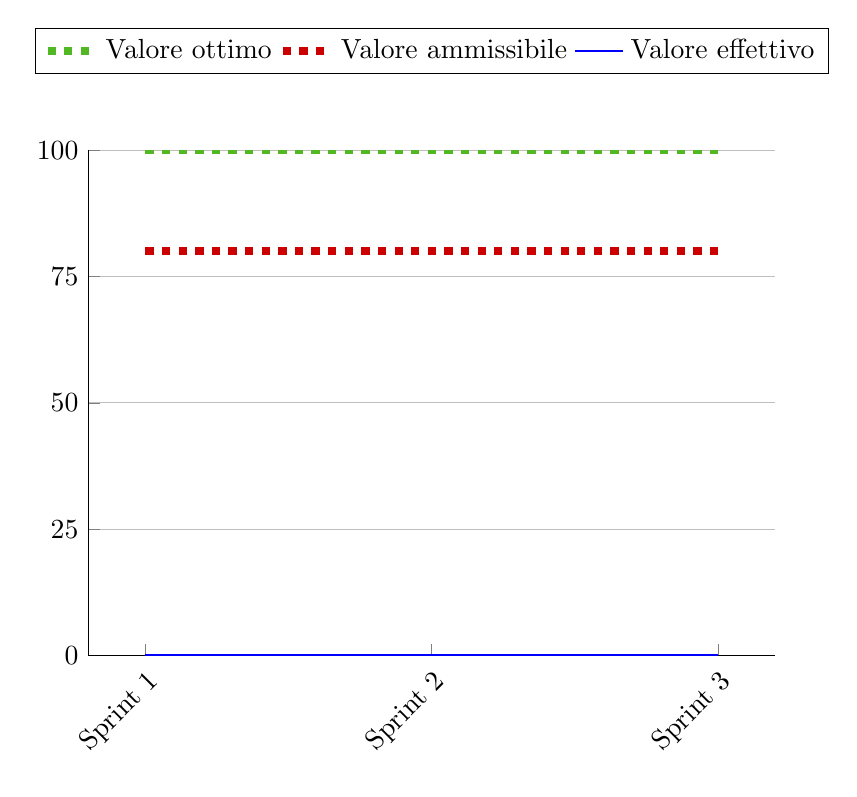
\begin{tikzpicture}
        \begin{axis}[
            width  = 0.85*\textwidth,
            height = 8cm,
            ymajorgrids = true,
            symbolic x coords={Sprint 1, Sprint 2, Sprint 3},
            xtick = data,
            ytick = {0, 25, 50, 75, 100},
            ymin=0, ymax=100,
            axis lines*=left,
            legend cell align=left,
            legend style={
                at={(0.5,1.15)},
                anchor=south,
                column sep=0.1ex,
                legend columns=3
            },      
            xticklabel style={rotate=45, anchor=north east, yshift=0ex, xshift=0ex}
            ]
            \addplot[color=opt, style={dashed, line width=3pt}, mark=none] coordinates {(Sprint 1, 100) (Sprint 2, 100) (Sprint 3, 100)};
            \addplot[color=amm, style={dashed, line width=3pt}, mark=none] coordinates {(Sprint 1, 80) (Sprint 2, 80) (Sprint 3, 80)};
            \addplot[color=blue, style={line width=1pt}, mark=none] coordinates {(Sprint 1, 0) (Sprint 2, 0) (Sprint 3, 0)};
            \legend{Valore ottimo, Valore ammissibile, Valore effettivo}
        \end{axis}
    \end{tikzpicture}
    \caption{Percentuale di branch coverage dei test implementati}
    \label{fig:11}
\end{figure*}
%--------- FINE GRAFICO -----------%
%\textbf{RTB} \\
% TODO considerazioni finali per RTB \\
%\textbf{PB} \\
% TODO considerazioni finali per PB

\newpage
\subsubsection{26M-SC - Statement coverage}
%--------- GRAFICO -----------%
\begin{figure*}[!h]
    \centering
    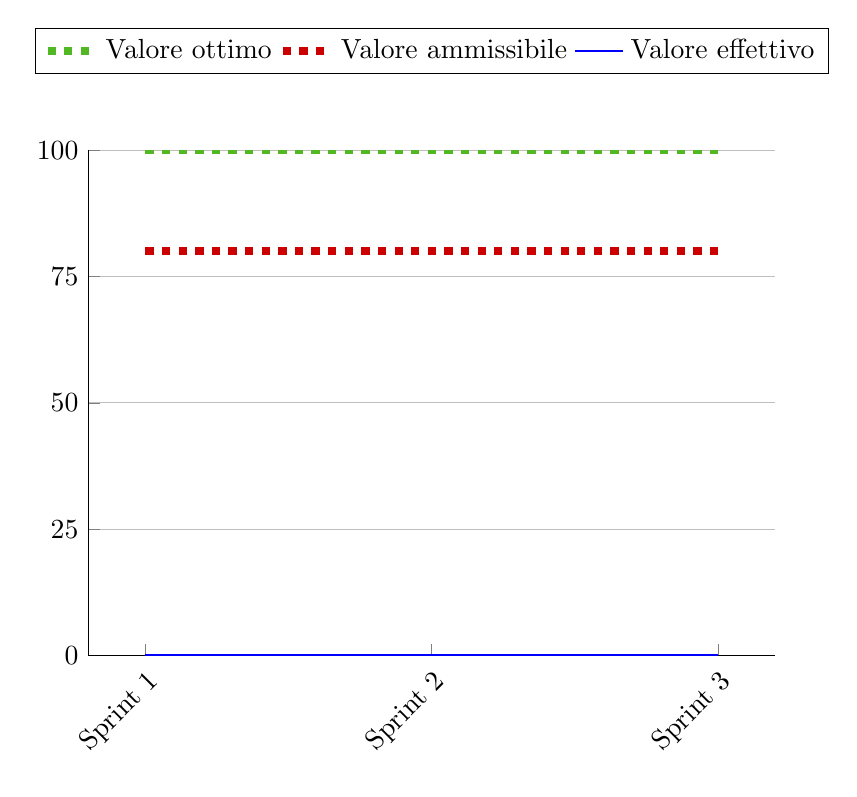
\begin{tikzpicture}
        \begin{axis}[
            width  = 0.85*\textwidth,
            height = 8cm,
            ymajorgrids = true,
            symbolic x coords={Sprint 1, Sprint 2, Sprint 3},
            xtick = data,
            ytick = {0, 25, 50, 75, 100},
            ymin=0, ymax=100,
            axis lines*=left,
            legend cell align=left,
            legend style={
                at={(0.5,1.15)},
                anchor=south,
                column sep=0.1ex,
                legend columns=3
            },      
            xticklabel style={rotate=45, anchor=north east, yshift=0ex, xshift=0ex}
            ]
            \addplot[color=opt, style={dashed, line width=3pt}, mark=none] coordinates {(Sprint 1, 100) (Sprint 2, 100) (Sprint 3, 100)};
            \addplot[color=amm, style={dashed, line width=3pt}, mark=none] coordinates {(Sprint 1, 80) (Sprint 2, 80) (Sprint 3, 80)};
            \addplot[color=blue, style={line width=1pt}, mark=none] coordinates {(Sprint 1, 0) (Sprint 2, 0) (Sprint 3, 0)};
            \legend{Valore ottimo, Valore ammissibile, Valore effettivo}
        \end{axis}
    \end{tikzpicture}
    \caption{Percentuale di statement coverage dei test implementati}
    \label{fig:12}
\end{figure*}
%--------- FINE GRAFICO -----------%
%\textbf{RTB} \\
% TODO considerazioni finali per RTB \\
%\textbf{PB} \\
% TODO considerazioni finali per PB

\newpage
\subsubsection{27M-FD - Failure density}
%--------- GRAFICO -----------%
\begin{figure*}[!h]
    \centering
    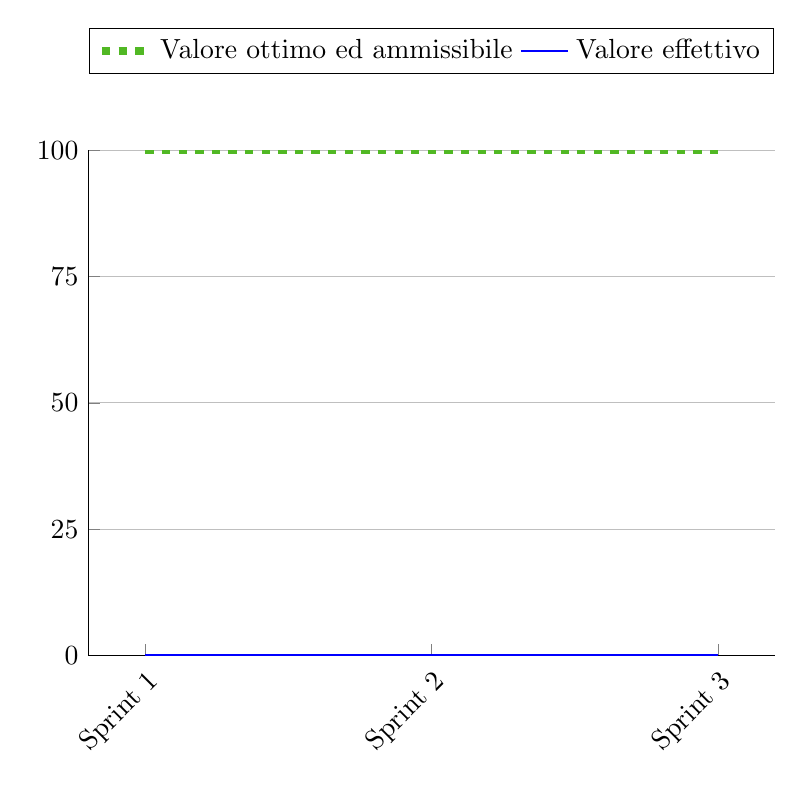
\begin{tikzpicture}
        \begin{axis}[
            width  = 0.85*\textwidth,
            height = 8cm,
            ymajorgrids = true,
            symbolic x coords={Sprint 1, Sprint 2, Sprint 3},
            xtick = data,
            ytick = {0, 25, 50, 75, 100},
            ymin=0, ymax=100,
            axis lines*=left,
            legend cell align=left,
            legend style={
                at={(0.5,1.15)},
                anchor=south,
                column sep=0.1ex,
                legend columns=3
            },      
            xticklabel style={rotate=45, anchor=north east, yshift=0ex, xshift=0ex}
            ]
            \addplot[color=opt, style={dashed, line width=3pt}, mark=none] coordinates {(Sprint 1, 100) (Sprint 2, 100) (Sprint 3, 100)};
            \addplot[color=blue, style={line width=1pt}, mark=none] coordinates {(Sprint 1, 0) (Sprint 2, 0) (Sprint 3, 0)};
            \legend{Valore ottimo ed ammissibile, Valore effettivo}
        \end{axis}
    \end{tikzpicture}
    \caption{Percentuale di failure density}
    \label{fig:13}
\end{figure*}
%--------- FINE GRAFICO -----------%
%\textbf{RTB} \\
% TODO considerazioni finali per RTB \\
%\textbf{PB} \\
% TODO considerazioni finali per PB

\newpage
\subsubsection{28M-PTCP - Passed Test Cases Percentage}
%--------- GRAFICO -----------%
\begin{figure*}[!h]
    \centering
    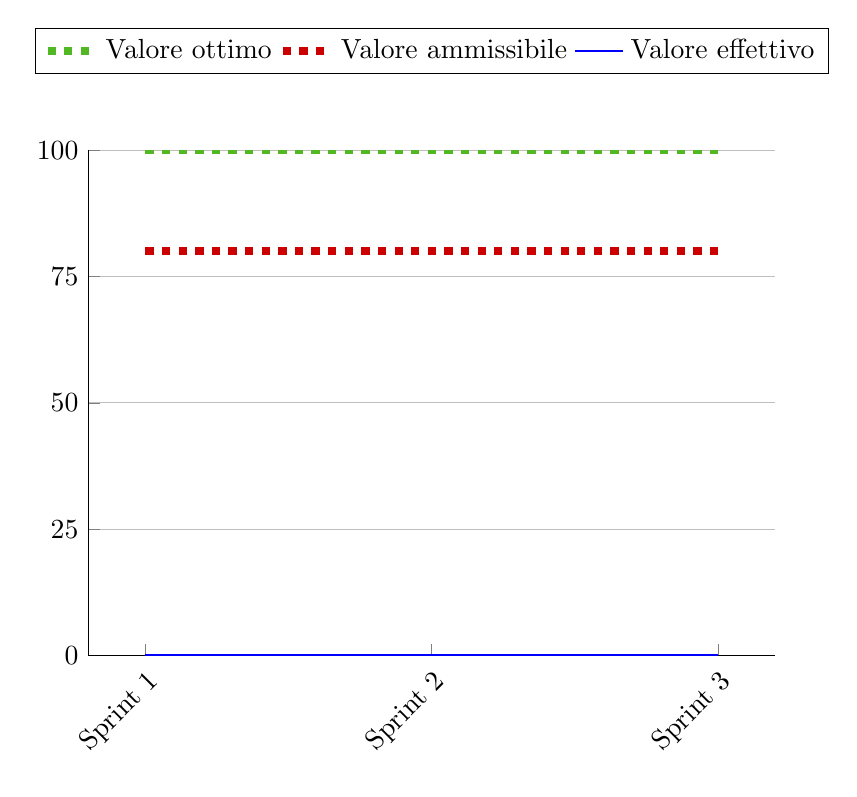
\begin{tikzpicture}
        \begin{axis}[
            width  = 0.85*\textwidth,
            height = 8cm,
            ymajorgrids = true,
            symbolic x coords={Sprint 1, Sprint 2, Sprint 3},
            xtick = data,
            ytick = {0, 25, 50, 75, 100},
            ymin=0, ymax=100,
            axis lines*=left,
            legend cell align=left,
            legend style={
                at={(0.5,1.15)},
                anchor=south,
                column sep=0.1ex,
                legend columns=3
            },      
            xticklabel style={rotate=45, anchor=north east, yshift=0ex, xshift=0ex}
            ]
            \addplot[color=opt, style={dashed, line width=3pt}, mark=none] coordinates {(Sprint 1, 100) (Sprint 2, 100) (Sprint 3, 100)};
            \addplot[color=amm, style={dashed, line width=3pt}, mark=none] coordinates {(Sprint 1, 80) (Sprint 2, 80) (Sprint 3, 80)};
            \addplot[color=blue, style={line width=1pt}, mark=none] coordinates {(Sprint 1, 0) (Sprint 2, 0) (Sprint 3, 0)};
            \legend{Valore ottimo, Valore ammissibile, Valore effettivo}
        \end{axis}
    \end{tikzpicture}
    \caption{Percentuale di casi di test superati}
    \label{fig:14}
\end{figure*}
%--------- FINE GRAFICO -----------%
%\textbf{RTB} \\
% TODO considerazioni finali per RTB \\
%\textbf{PB} \\
% TODO considerazioni finali per PB

\newpage
\subsection{Qualità del processo di Gestione dei rischi}
\subsubsection{29M-NCR - Non-Calculated Risk}
%--------- GRAFICO -----------%
\begin{figure*}[!h]
    \centering
    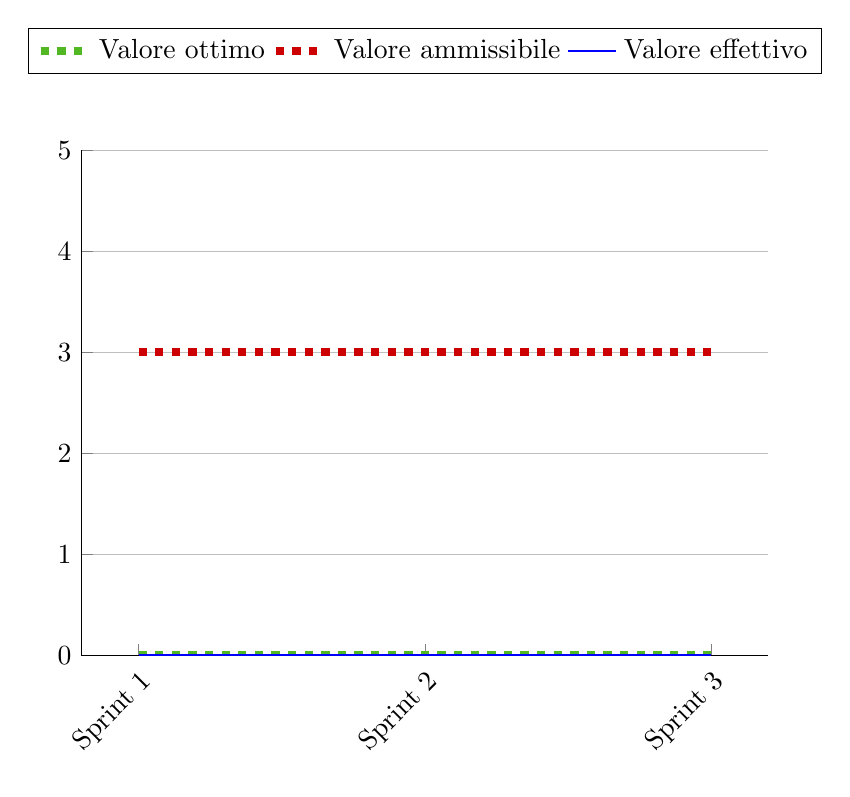
\begin{tikzpicture}
        \begin{axis}[
            width  = 0.85*\textwidth,
            height = 8cm,
            ymajorgrids = true,
            symbolic x coords={Sprint 1, Sprint 2, Sprint 3},
            xtick = data,
            ymin=0, ymax=5,
            axis lines*=left,
            legend cell align=left,
            legend style={
                at={(0.5,1.15)},
                anchor=south,
                column sep=0.1ex,
                legend columns=3
            },      
            xticklabel style={rotate=45, anchor=north east, yshift=0ex, xshift=0ex}
            ]
            \addplot[color=opt, style={dashed, line width=3pt}, mark=none] coordinates {(Sprint 1, 0) (Sprint 2, 0) (Sprint 3, 0)};
            \addplot[color=amm, style={dashed, line width=3pt}, mark=none] coordinates {(Sprint 1, 3) (Sprint 2, 3) (Sprint 3, 3)};
            \addplot[color=blue, style={line width=1pt}, mark=none] coordinates {(Sprint 1, 0) (Sprint 2, 0) (Sprint 3, 0)};
            \legend{Valore ottimo, Valore ammissibile, Valore effettivo}
        \end{axis}
    \end{tikzpicture}
    \caption{Rischi non calcolati occorsi durante il progetto}
    \label{fig:15}
\end{figure*}
%--------- FINE GRAFICO -----------%
%\textbf{RTB} \\
% TODO considerazioni finali per RTB \\
%\textbf{PB} \\
% TODO considerazioni finali per PB

\newpage
\subsection{Qualità del processo di Gestione della qualità}
\subsubsection{30M-QMS - Quality Metrics Satisfied}
%--------- GRAFICO -----------%
\begin{figure*}[!h]
    \centering
    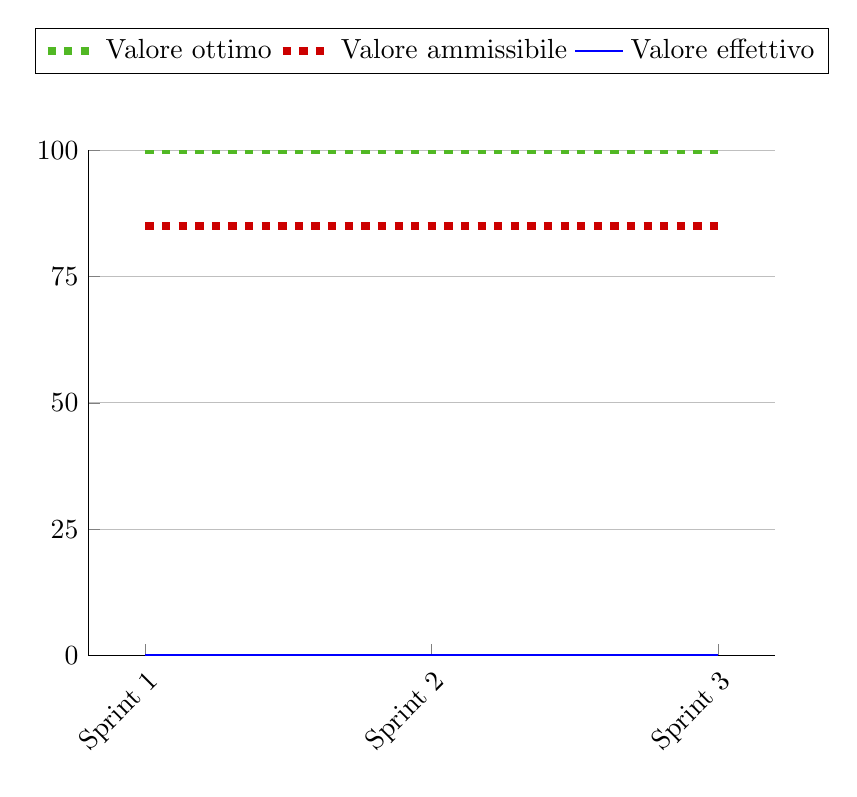
\begin{tikzpicture}
        \begin{axis}[
            width  = 0.85*\textwidth,
            height = 8cm,
            ymajorgrids = true,
            symbolic x coords={Sprint 1, Sprint 2, Sprint 3},
            xtick = data,
            ytick = {0, 25, 50, 75, 100},
            ymin=0, ymax=100,
            axis lines*=left,
            legend cell align=left,
            legend style={
                at={(0.5,1.15)},
                anchor=south,
                column sep=0.1ex,
                legend columns=3
            },      
            xticklabel style={rotate=45, anchor=north east, yshift=0ex, xshift=0ex}
            ]
            \addplot[color=opt, style={dashed, line width=3pt}, mark=none] coordinates {(Sprint 1, 100) (Sprint 2, 100) (Sprint 3, 100)};
            \addplot[color=amm, style={dashed, line width=3pt}, mark=none] coordinates {(Sprint 1, 85) (Sprint 2, 85) (Sprint 3, 85)};
            \addplot[color=blue, style={line width=1pt}, mark=none] coordinates {(Sprint 1, 0) (Sprint 2, 0) (Sprint 3, 0)};
            \legend{Valore ottimo, Valore ammissibile, Valore effettivo}
        \end{axis}
    \end{tikzpicture}
    \caption{Percentuale di metriche di qualità soddisfatte}
    \label{fig:16}
\end{figure*}
%--------- FINE GRAFICO -----------%
%\textbf{RTB} \\
% TODO considerazioni finali per RTB \\
%\textbf{PB} \\
% TODO considerazioni finali per PB

\newpage
\subsubsection{31M-TE - Efficienza Temporale}
%--------- GRAFICO -----------%
\begin{figure*}[!h]
    \centering
    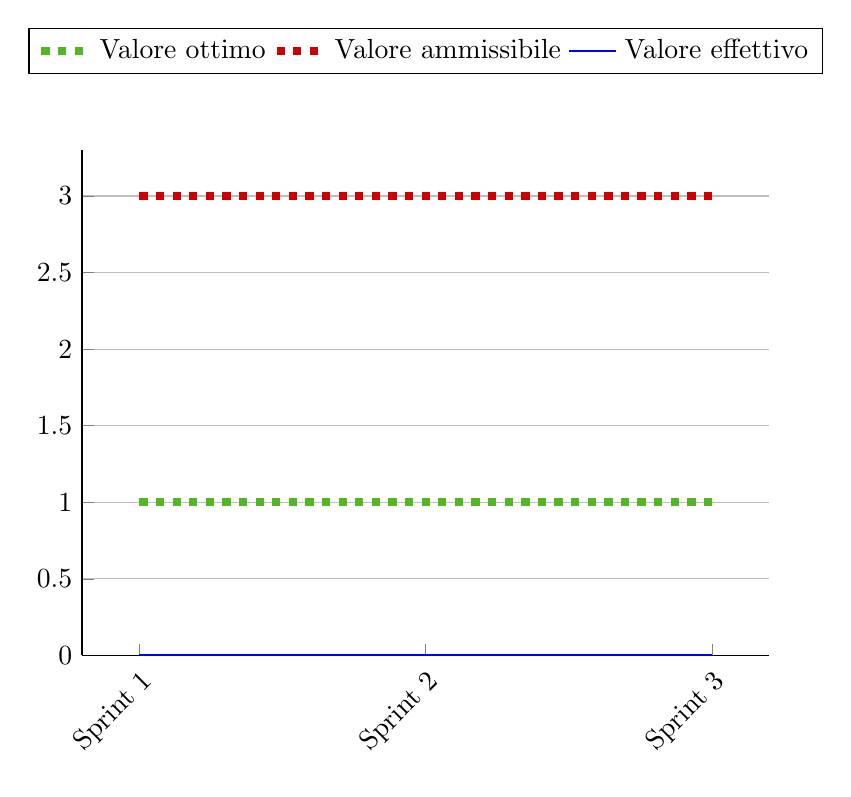
\begin{tikzpicture}
        \begin{axis}[
            width  = 0.85*\textwidth,
            height = 8cm,
            ymajorgrids = true,
            symbolic x coords={Sprint 1, Sprint 2, Sprint 3},
            xtick = data,
            ymin=0,
            axis lines*=left,
            legend cell align=left,
            legend style={
                at={(0.5,1.15)},
                anchor=south,
                column sep=0.1ex,
                legend columns=3
            },      
            xticklabel style={rotate=45, anchor=north east, yshift=0ex, xshift=0ex}
            ]
            \addplot[color=opt, style={dashed, line width=3pt}, mark=none] coordinates {(Sprint 1, 1) (Sprint 2, 1) (Sprint 3, 1)};
            \addplot[color=amm, style={dashed, line width=3pt}, mark=none] coordinates {(Sprint 1, 3) (Sprint 2, 3) (Sprint 3, 3)};
            \addplot[color=blue, style={line width=1pt}, mark=none] coordinates {(Sprint 1, 0) (Sprint 2, 0) (Sprint 3, 0)};
            \legend{Valore ottimo, Valore ammissibile, Valore effettivo}
        \end{axis}
    \end{tikzpicture}
    \caption{Andamento dell'efficienza temporale}
    \label{fig:17}
\end{figure*}
%--------- FINE GRAFICO -----------%
%\textbf{RTB} \\
% TODO considerazioni finali per RTB \\
%\textbf{PB} \\
% TODO considerazioni finali per PB

\newpage
\subsection{Qualità del processo di Pianificazione}
\subsubsection{32M-RSI - Requirements stability index (RSI)}
%--------- GRAFICO -----------%
\begin{figure*}[!h]
    \centering
    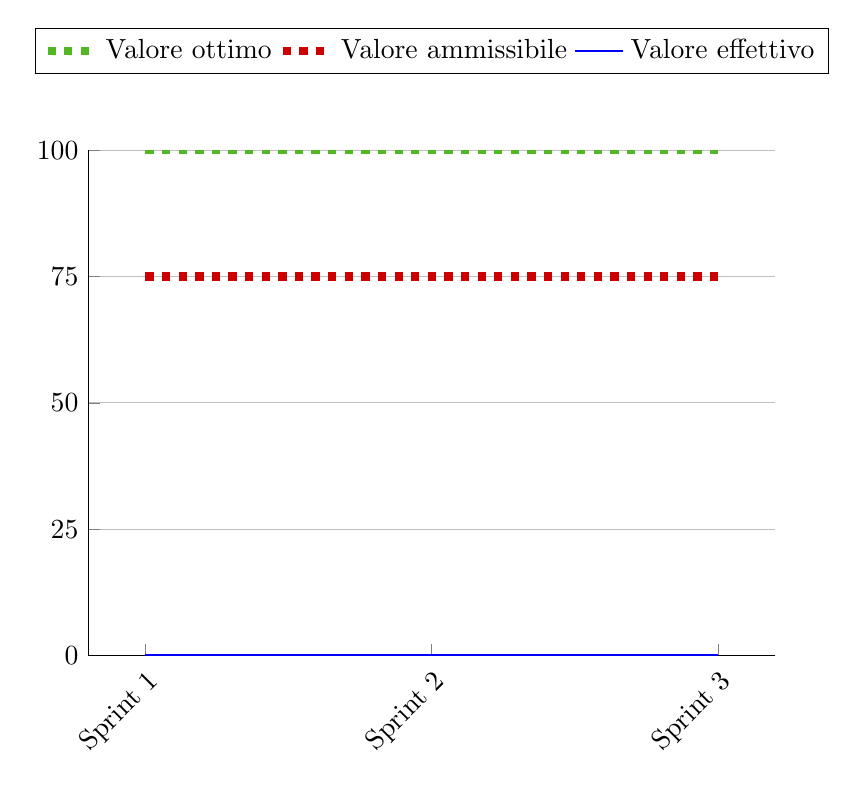
\begin{tikzpicture}
        \begin{axis}[
            width  = 0.85*\textwidth,
            height = 8cm,
            ymajorgrids = true,
            symbolic x coords={Sprint 1, Sprint 2, Sprint 3},
            xtick = data,
            ytick = {0, 25, 50, 75, 100},
            ymin=0, ymax=100,
            axis lines*=left,
            legend cell align=left,
            legend style={
                at={(0.5,1.15)},
                anchor=south,
                column sep=0.1ex,
                legend columns=3
            },      
            xticklabel style={rotate=45, anchor=north east, yshift=0ex, xshift=0ex}
            ]
            \addplot[color=opt, style={dashed, line width=3pt}, mark=none] coordinates {(Sprint 1, 100) (Sprint 2, 100) (Sprint 3, 100)};
            \addplot[color=amm, style={dashed, line width=3pt}, mark=none] coordinates {(Sprint 1, 75) (Sprint 2, 75) (Sprint 3, 75)};
            \addplot[color=blue, style={line width=1pt}, mark=none] coordinates {(Sprint 1, 0) (Sprint 2, 0) (Sprint 3, 0)};
            \legend{Valore ottimo, Valore ammissibile, Valore effettivo}
        \end{axis}
    \end{tikzpicture}
    \caption{Percentuale di cambiamento dei requisiti}
    \label{fig:18}
\end{figure*}
%--------- FINE GRAFICO -----------%
%\textbf{RTB} \\
% TODO considerazioni finali per RTB \\
%\textbf{PB} \\
% TODO considerazioni finali per PB
